\documentclass[12pt]{article}

\usepackage{graphicx}
\usepackage{amsmath}
\usepackage{amssymb}
\usepackage{natbib}
\usepackage{amsfonts}
\usepackage{multicol}
\usepackage{float}
\usepackage{oldgerm}
\usepackage{bm}
\usepackage{mathtools}
\usepackage{wrapfig}
\usepackage{fancyhdr}
\usepackage[export]{adjustbox}
\usepackage{xcolor}
\usepackage[shortlabels]{enumitem}

\pagestyle{empty}

\setlength{\headsep}{0.5cm}
\setlength{\oddsidemargin}{-0.5cm}
\setlength{\textwidth}{16.5cm}
\setlength{\textheight}{24cm}
\voffset = -2cm


\pagestyle{fancy}
\fancyhf{}
\rfoot{
\includegraphics[width=1.0in]{cnm.png}}
\lfoot{Homework 3}
\setlength\parindent{0pt}
\begin{document}

\begin{center}
\hfil
{\large\bf {ENGR 2910-101: Circuit Analysis}}
\hfill Instructor: Brian Rashap\\
Homework 3: 01/25/23 \hfill Due: 02/01/23\\
\hrulefill\\
\end{center}

{\bf Question 1} [10] %P3-3

For each of the circuits (a)-(d), find the equivalent resistance and the power delivered by the source. 
\begin{figure}[h!]
  \centering 
 \vspace{-0.1in}
 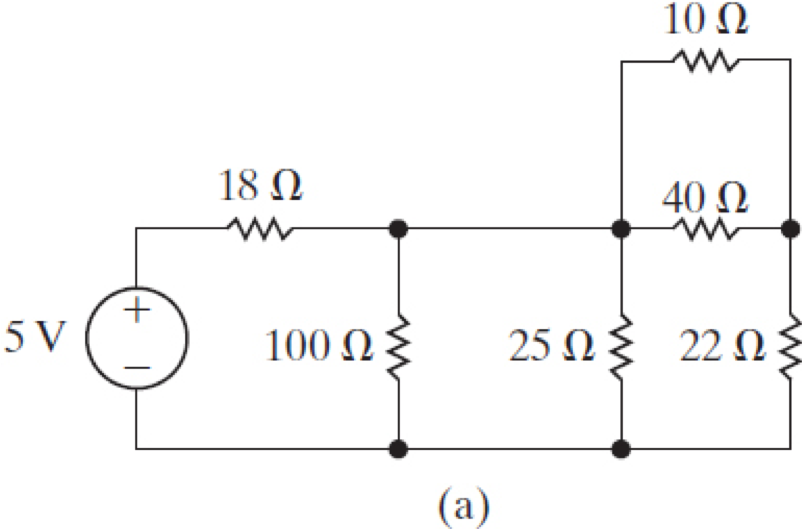
\includegraphics[clip,width=0.45\textwidth]{Fig3-3a.png}
 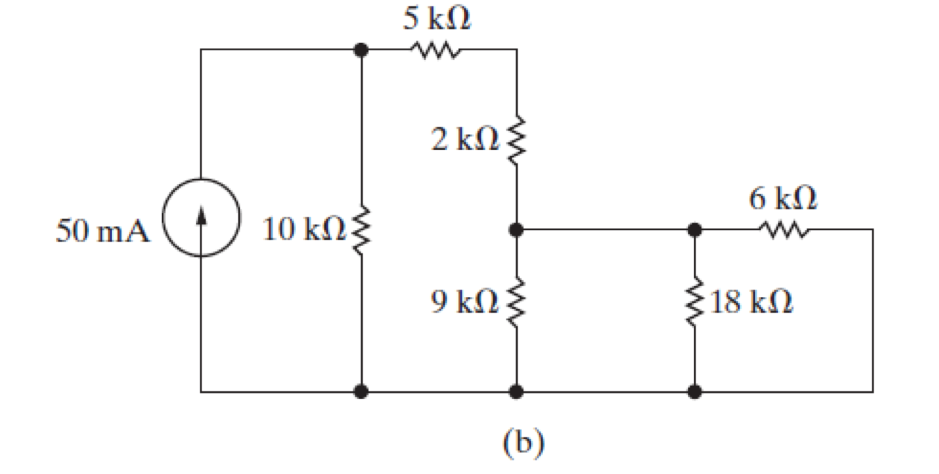
\includegraphics[clip,width=0.45\textwidth]{Fig3-3b.png}\\
 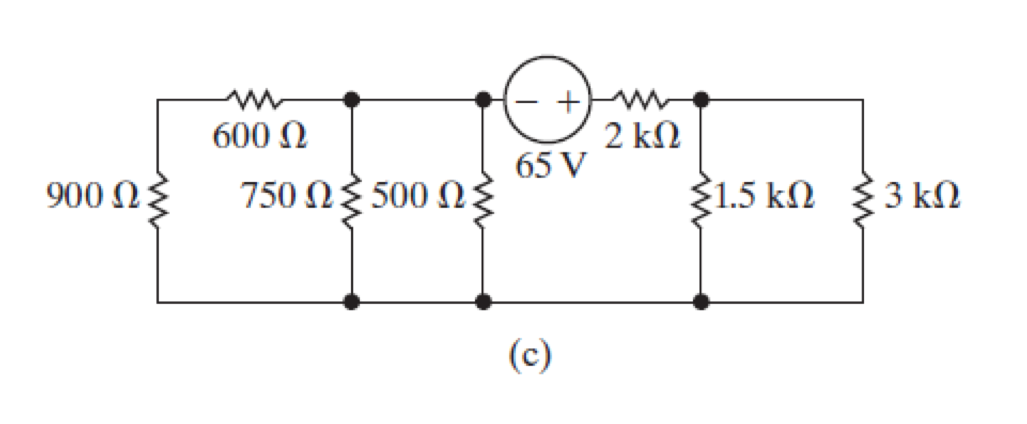
\includegraphics[clip,width=0.45\textwidth]{Fig3-3c.png}
 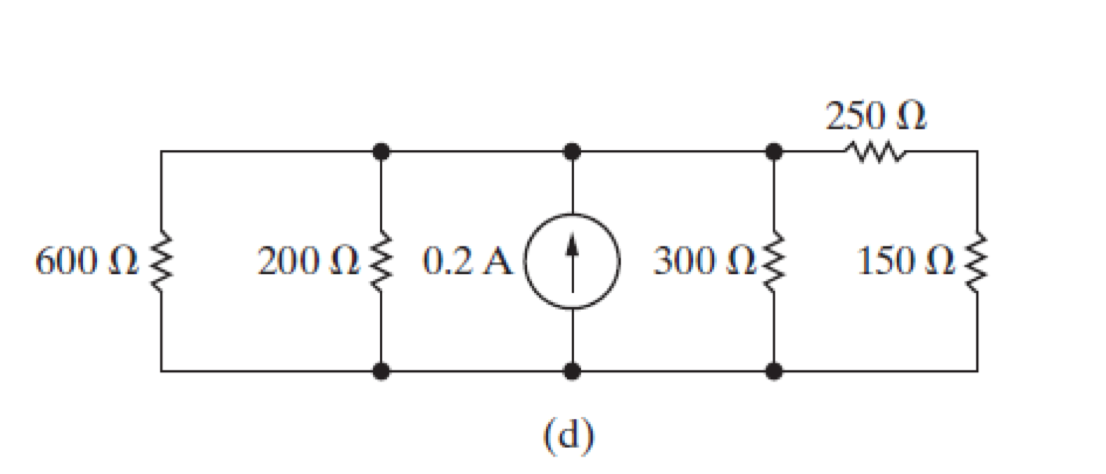
\includegraphics[clip,width=0.45\textwidth]{Fig3-3d.png}
%\vspace{-0.1in}
\end{figure}

\vspace{0.1in}
\noindent
{\bf Question 2} [10] %P3-6(d)

Find the equivalent resistance $R_{ab}$ for the following circuit.
\begin{figure}[h!]
     \centering
\vspace{-0.1in}
     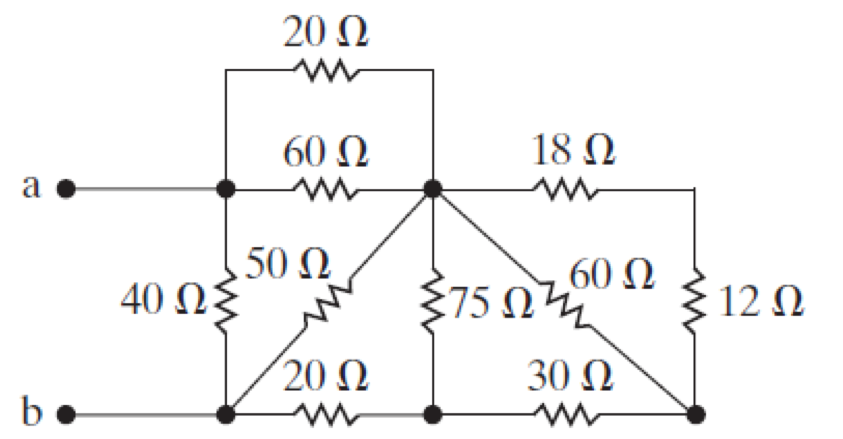
\includegraphics[clip,width=0.6\textwidth]{Fig3-6d.png}
\vspace{-0.15in}
\end{figure}
 \newpage
\noindent
{\bf Question 3} [10] %openstax

A battery of 45 V delivers 112 W of power to the circuit that contains 5 identical resistors (R$_{i}$=R). What is the value of R?

\begin{figure}[!h]
  \centering 
  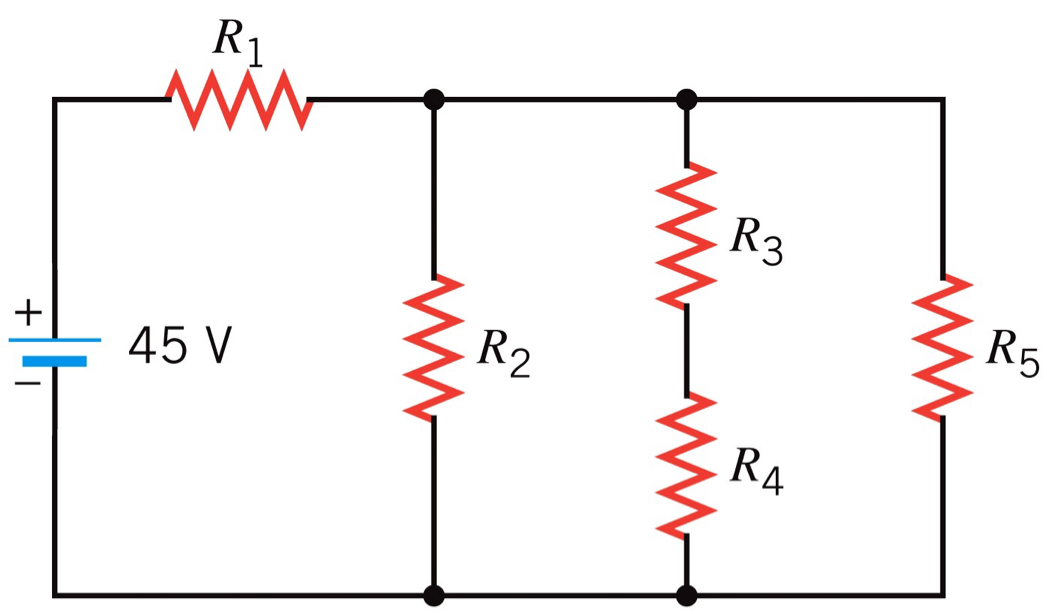
\includegraphics[clip,width=0.4\textwidth]{Fig-Q3.png}
\end{figure}

\vspace{0.1in}
\noindent
{\bf Question 4} [10] %P3-13

For the voltage-divider circuit shown: 
\begin{figure}[h!]
  \centering 
  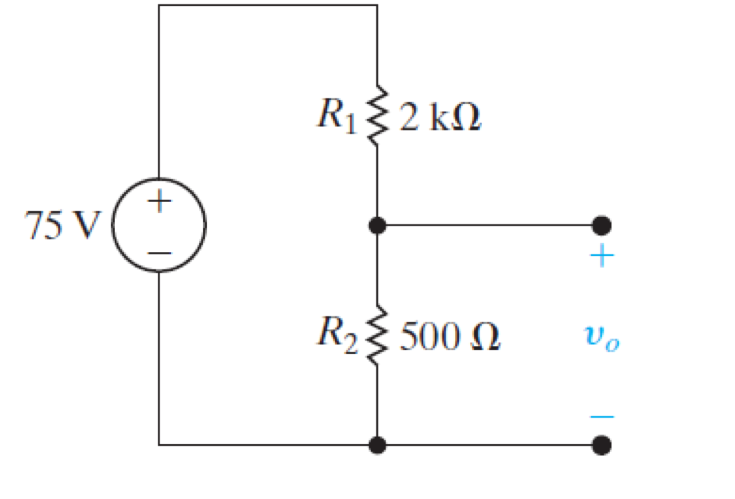
\includegraphics[clip,width=0.4\textwidth]{Fig3-13.png}
\end{figure}

\begin{enumerate}[(a)]
\item Calculate the no-load voltage $v_{o}$.
\item Calculate the power dissipated in $R_{1}$ and $R_{2}$.
\item If only 1 W resistors are available and that the no-load voltage is to be the same as in part (a), specify the smallest values of $R_{1}$ and $R_{2}$.
\end{enumerate}


\vspace{0.1in}
\noindent
{\bf Question 5} [10] %P3-58

Use a $\Delta$-to-{\bf Y} transformation to find the voltages $v_1$ and $v_2$ int he circuit below.
\begin{figure}[h!]
\centering 
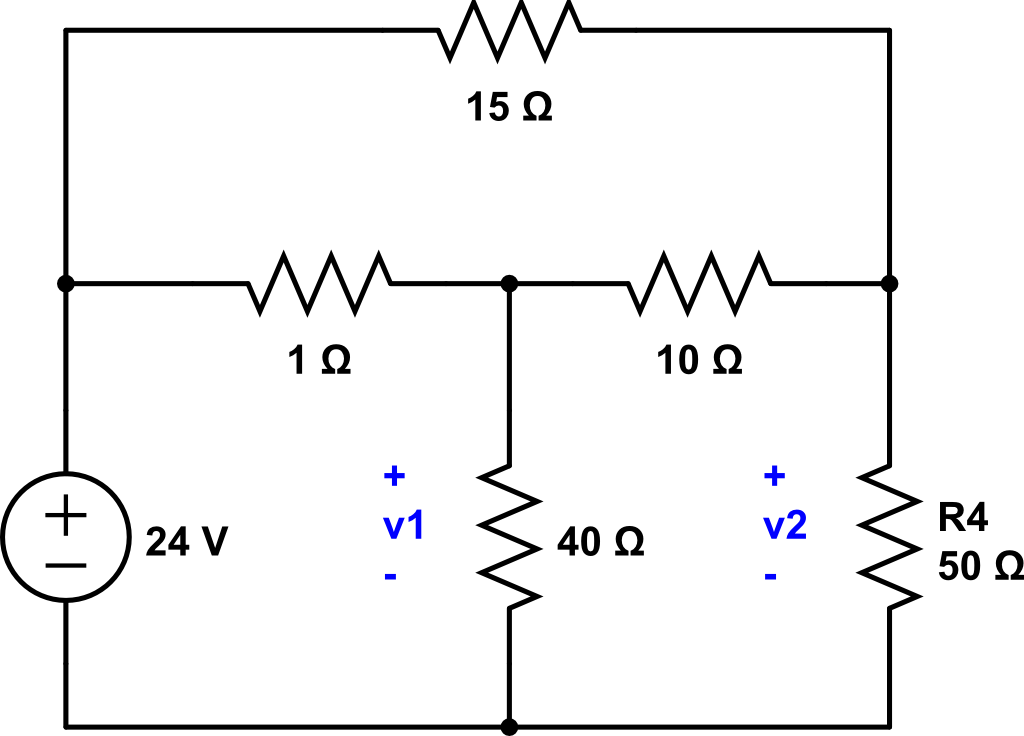
\includegraphics[clip,width=0.4\textwidth]{Fig3_58.png}
\end{figure}
 
\end{document}
